% !TEX root = ../Thesis.tex
%%
%%  Hochschule für Technik und Wirtschaft Berlin --  Abschlussarbeit
%%
%% Kapitel 2 - Grundlagen
%%
%%


\chapter{Grundlagen} \label{Grundlagen}



\section{Begriffserklärungen}

Da \textbf{\textit{Klärwerke}} hinsichtlich ihrer Funktion in der Informatik grundsätzlich selten betrachtet werden, wird im folgenden die Quintessenz für die Betrachtung der Problemstellung aufgebaut. Hierbei geht es insbesondere um grundsätzliche Bestandteile, aber auch lokal spezifische Gegebenheiten, die technisch, chemisch und informationselektronisch dargelegt werden.

Die Grundlagen für Faltbare Neuronale Netzwerke (CNNs) werden erläutert, wobei auch auf die zugrunde liegende Mathematik eingegangen wird. Zusätzlich erfolgt eine tabellarische Aufführung der Datensätze, der Arten von Neuronalen Netzwerken und den Verfahren zur Segmentierung zur Übersichtlichkeit. 

Um die später vorgestellten Übertragungstechniken und Kommunikationstechnologien besser einordnen zu können, wird zu Beginn auf das OSI-Modell \index{OSI-Modell}eingegangen.

Außerdem werden weitere Begriffe erläutert, die helfen sollen, die zu implementierende Lösung einzugruppieren. Teilweise handelt es sich um englische Begriffe, weil diese auch in der deutschen Literatur gebräuchlicher sind.

\subsection{Klärwerk}

In Klärwerken wird das ankommende Abwasser in mehreren Schritten geklärt. Angefangen mit mechanischen Reinigungsprozessen wie dem Grobrechen, der größere Bestandteile aus dem Wasser herausfiltert, den Sand- und Fettfängen, deren Zweck die Nutzung von Sedimentationsverfahren zur physischen Trennung von Lipiden und lockeren Gesteinsmaterialien ist. Anschließend werden Belebungslinien eingesetzt, die das Bakterienwachstum fördern sollen, um die Verarbeitung des Klärwassers voranzutreiben. Hierfür durchläuft das kommunale Abwasser mehrere Phasen, in denen mittels aerober Mikroorganismen die organischen Verunreinigungen verstoffwechselt werden. \cite{Jenkins_2004} \\
Am Ende dieser biologischen Prozesse wird das Wasser in Nachklärbecken weitergeleitet, die dieses in 4 Zonen unterteilt: Klarwasser-, Trenn-, Speicher- und Räum-/Eindickzone. Mittels sogennanter Räumer wird das Wasser gleichmäßig verteilt und der gram-positive Schlamm am Beckengrund in der Eindickzone abgeführt. Darüber befinden sich Speicher- und Trennzone, in denen sich die Partikel absetzen oder wie im Fall der gram-negativen Fadenorganismen auf der Klarwasserzone anreichern, wo sie Klär-/Blähschlamm bilden. Diese Art Schlamm wird ebenfalls gereinigt, da das übermäßige Wachstum zu einer Verdickung der Schicht führt. Das kann bewirken, dass der Ablauf des Klarwassers verschmutzt wird, weil sich die Schichten vermischen. Hierdurch entstehen weitere Probleme in der Klärung des Wassers, da die Qualitätsansprüche für (beispielsweise) eine Flockungsfiltration nicht erfüllt werden. \\ \\

\index{SSR}: Schwimmende-Schwimmschlamm-Räumer werden eingesetzt um über eine oder mehrere Förderschnecken den Oberflächenbelag an einem Schwimmschlamm-Schlürftrichter zu konzentrieren. Der Inhalt wird abgefördert, um die Oberfläche sauber zu halten, damit der Anteil an entsprechenden Fadenbakterien wie Microthrix Parvicella nicht überhand nimmt und das Gleichgewicht des Beckens stört.
Die bisherige Steuerung funktioniert über einen Timer, der zwischen Winter- und Sommerbetrieb umgeschalten wird, um auf die Veränderungen des Bakterienwachstums und der damit einhergehenden Oberflächen-
beschaffenheit annäherungsweise einzugehen. Da die biologischen Begebenheiten hierbei deutlich komplexer als ein simpler Zeitintervall sind, ergibt sich ein Optimierungsgedanke. 

\subsection{Neuronale Netzwerke}
Bereits im Jahr 1842 wurden programmierbare Rechner mit der Fähigkeit zur (menschlichen) Intelligenz erdacht, obwohl sie als einfache Maschinen erst über ein Jahrhundert später ins Leben gerufen wurden. Entsprechend alt ist der Grundgedanke von Apparaturen, die in ihren Zügen menschliche Denkeigenschaften verkörpern.
\cite{goodfellow_2016} \\ \\
Inzwischen hat sich viel getan über die anfänglichen Entwicklungen mit cybernetics in den 1940-60er Jahre als Entwicklung von Theorien zu biologischem Lernen und ersten Implementierungen zum Training eines einzelnen Neuronen mit dem \say{perceptron}, über connectionism, der mittels back-propagation das Training eines neuronalen Netzwerks mit ein oder zwei hidden layers ermöglichte und der aktuellen deep learning Entwicklung, die sich seit 2006 fortsetzt. \cite{Kim_2016} \\ \\
Mathematisch betrachtet liegen hier drei unterschiedliche Modelle vor. Die Ursprünge liegen im maschinellen Lernen, was hier in seinen Grundzügen erklärt sei. Beginnend mit dem Lernalgorithmus, der Grundzüge des Trainings auf Basis der Daten beschreibt. Eine allgemeine Definition von Tom Mitchell lautet: \say{A computer program is said to learn from experience \textbf{E} with respect to some class of tasks \textbf{T} and performance measure \textbf{P}, if its performance at tasks in \textbf{T}, as measured by \textbf{P}, improves with experience \textbf{E}.} 
Der Ausgestaltung der jeweiligen Kategorien werden nur von der Fantasie Grenzen gesetzt,was sich in differenzierten Ansätzen widerspiegelt. 

\subsubsection{Deep Learning}
Künstliche Intelligenz und Neuronale Netze stellen seit einigen Jahren den Status Quo dar, weswegen diese Technologie jedem ein Begriff sein sollte. Dennoch sei die grundlegende Funktionsweise hier erklärt, um das Basiswissen zu vereinheitlichen: 

\subsubsection{Semantische Segmentierung}
Die Semantische Segmentierung ist ein Konzept der Computer Vision, bei dem das erfasste Bild in mehrere Labels unterteilt wird. Nebeneinander liegende Pixel werden anhand von Alleinstellungsmerkmalen zusammengefasst.  Dieses Verfahren unterscheidet sich durch die strikte Aufteilung in allgemeine Schichten, während einzelne Objekte im Gegensatz zur Instanzsegmentierung oder panoptischen Segmentierung keine Rolle spielen. \cite{goodfellow_2016}

\begin{figure}[h]
    \centering
    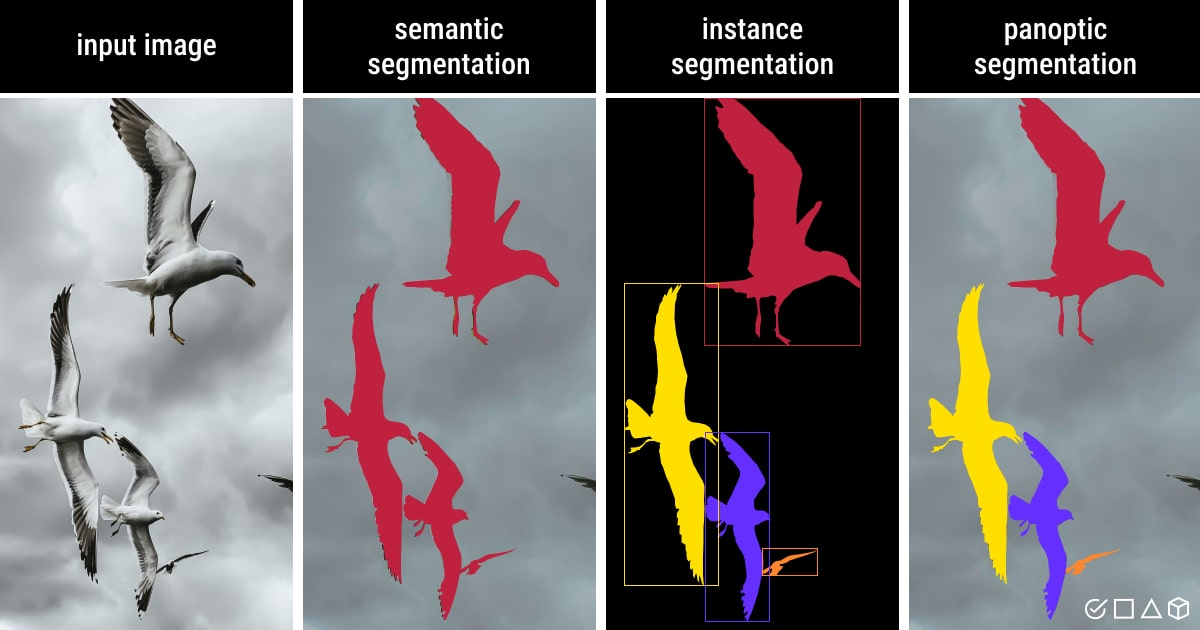
\includegraphics[width=0.8\linewidth]{pictures/segmentation_in_practice.jpg}
    \caption{Darstellung
    der Segmentierungsoptionen \cite{naminas_semantic_nodate} }
    \label{fig:Beispiel Segmentierung}
\end{figure}



\subsubsection{En- und Decoder}

En- und Decoder werden zur Verarbeitung sequentiellener Daten verwendet, bei denen es sich oft um sprachorientierte Modelle handelt. Hierbei werden Eingabesequenzen auf Ausgabesequenzen mit divergierender Länge übersetzt bzw. zugewiesen. In der Sprachübersetzung werden so anhand von trainierten Satzstrukturen Text aus dem Deutschen in das Englisch übersetzt, indem die Ausgabesequenz hinsichtlich ihrer Länge kontextuell modifizert wird.   

\begin{figure}[h]
    \centering
    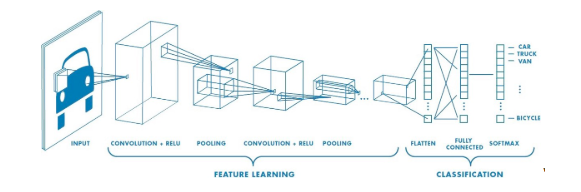
\includegraphics[width=0.8\linewidth]{pictures/De- und Encoder_hs_analysis.png}
    \caption{Darstellung der Verarbeitung von Encoder zu Decoder}
    \cite{}
    \label{fig:DeEncoder}
\end{figure}

Die Übersetzung erfolgt seitens des Encoders von dem ursprünglichen Datentyp hin zu einem vektoriellen und wird seitens des Decoders wieder zu zurückgewandelt. 
Sowohl De- als auch Encoder sind hierbei eigenständige Neuronale Netze, die in unterschiedlichen Varianten vorkommen können.
Die Basis eines Encoders ist ein zweischichtiges System, was sich einersauts aus einem Mechanismus zur Selbstüberwachung speist, der für die Gewichtung der Eingabe und damit der einzelnen Token und ihren Zusammenhang zuständig ist. 

\begin{equation}
    x_i = \sum_{j=1}^nw_{ji}x_{j}
\end{equation}

$x_j$ markiert hierbei einen eingegebenen Token (Wort) mit dem Index j in dem Eingabetext, während $x_i$ dem ausgegebenen Token mit dem Index i im Ausgabetext entspricht. Der Koeffizient $w_{ij}$ stellt die per Softmax-Funktion berechnete Gewichtung dar und damit die Wichtigkeit des Tokens für den Ausgabetext definiert. Manche Wortarten wie Verben haben zum Beispiel eine höhere Aussagekraft und dementsprechend Gewichtung als Füllwörter oder Artikel. Gleiches gilt in der Bildverarbeitung für die Kategorisierung einzelner Pixel in Hinblick auf ihre Klasse und der damit verbundenen Auswirkung auf Verarbeitung.  

Anschließend wird der entsprechende Token durch die Feed-Forward-Schicht eingebettet, was einer Positionskodierung in einem Satz anhand des Index (z.B. LLM) oder einer Einordnung in ein pixelweises, zweidimensionales Koordinatensystem entspricht (CNN, Bildverarbeitung). Aus beiden Schichten setzt sich der verborgene Zustand (Kontextvektor) zusammen, der als ein Element an den Decoder weitergegeben wird.

\begin{figure}[h]
    \centering
    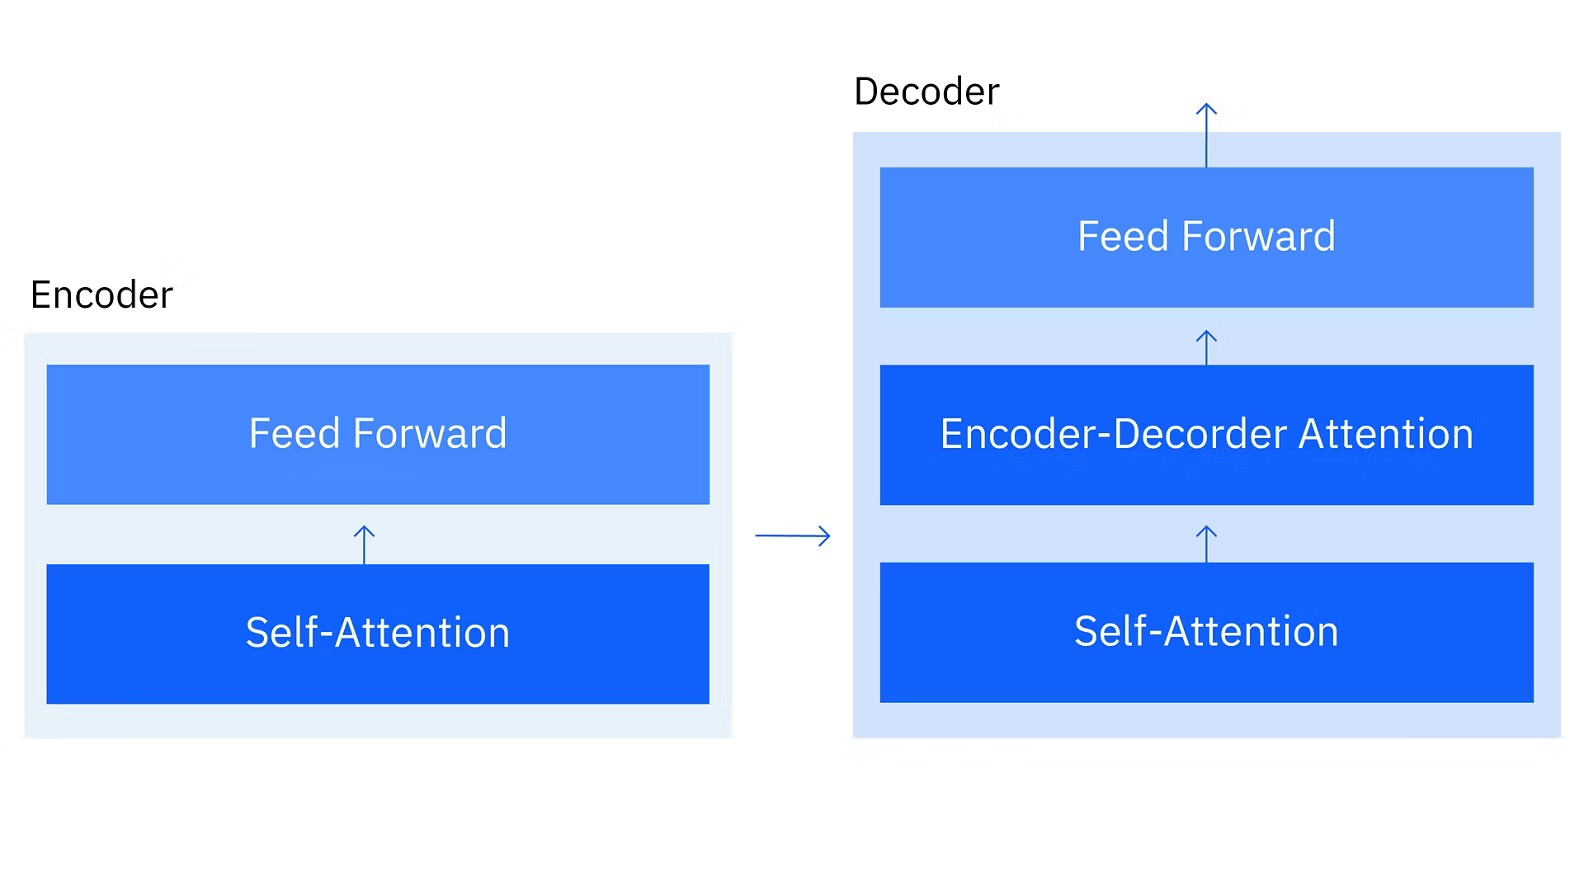
\includegraphics[width=0.8\linewidth]{pictures/encoder-decoder-image_ibm.png}
    \caption{Caption}
    \label{fig:Encoder-Decoder}
\end{figure}

Eine klassische Encoder-/Decoder-Architektur ist das U-Net. Dabei handelt es sich um eine Weiterentwicklung des FCNN mit dem Ziel, Bildsegmentierung mit kleinen Datensätzen und dennoch hoher Präzision zu verarbeiten. Wie der Name bereits andeutet, ist diese Architektur U-förmig aufgebaut: durch die hohe Anzahl an Kanälen, die Eigenschaften extrahieren, ist der kontrahierende Pfad ähnlicher Länge wie der expandierende. \cite{Ronneberger_2015} Dieses Verfahren wurde auch in diesem Projekt verwendet, um die Arbeit mit geringen Datenmengen zu vereinfachen und zugleich die Perfomanz hoch zu halten. Ein weiterer Vorteil besteht in der Nutzung von Skip-Connections, also dem partiellen Überspringen von Layern um qualitative Bilddetails zu erhalten.

\begin{figure}[h]
    \centering
    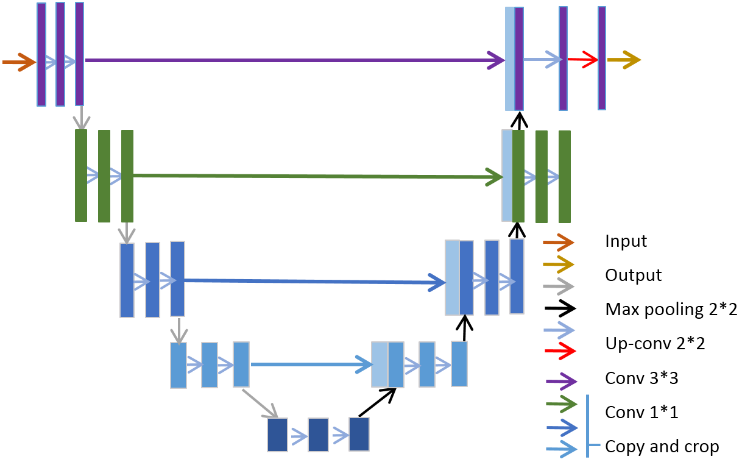
\includegraphics[width=0.5\linewidth]{pictures/The-architecture-of-Unet_researchgate.png}
    \caption{Caption}
    \label{fig:placeholder}
    \cite{Howard_2017}
\end{figure}


\textbf{Abschnitt schärfen:} U-Net als Encoder-Decoder-Architektur erklären (Skip-Connections, warum gut für Segmentierung) und passende Quelle(n) zitieren.

\subsubsection{Programme }

\subsection{Formeln}


Bayes Theorem
\begin{equation}
    Pr(H|E) = \frac{Pr(E|H)Pr(H)}{Pr(E|H)Pr(H) + Pr(E|!H)Pr(!H)}
\end{equation}

Das Bayes-Theorem dient der Berechnung der bedingten Wahrscheinlichkeit, dass A eintritt, wenn B bereits eingetreten ist, unter der Voraussetzung dass die Wahrscheinlichkeit von B unter der Bedingung von A vorliegt. 

Grundsätzlich ermöglicht dieser Satz also die Berechnung des Ereignisses $Pr(H|E)$ auf Grundlage von $Pr(E|H)$ mit dem Satz der totalen Wahrscheinlichkeit. 

Softmax-Funktion
\begin{equation}
    softmax(x)_i=\frac{e^{(x_i)}}{\Sigma_{j=1}^ne^{(x_j)}}
\end{equation}

Mittels der Softmax-Funktion wird ein Vektor als Input zu Wahrscheinlichkeiten überführt, deren Größe direkt damit korreliert. Ein hoher numerischer Wert geht mit einer entsprechenden Wahrscheinlichkeit einher. Mittels dieser Funktion wird dafür gesorgt, dass folgendes für die Summe der Ausgabewerte $S_a$ gilt: $S_a \leq 1$
Dieser Aspekt ist von hoher Relevanz für die Wahrscheinlichkeitsrechnung, in der nur dieses Spektrum für die Wahrscheinlichkeit von Interesse ist.

Schwellwertfunktion
\begin{equation}
     f(x)=\left\{\begin{array}{ll} 1, & x \geq a \\
         0, & sonst\end{array}\right. .
\end{equation}

Sigmoid-Funktion
\begin{equation}
     f(x)=\frac{1}{1+e^{-x}}
\end{equation}

ReLU
\begin{equation}
     f(x)=\left\{\begin{array}{ll} x & x \geq 0 \\
         0, & sonst\end{array}\right. .
\end{equation}

Eine Rectified Linear Unit Funktion entspricht einer Aktivierungsfunktion, deren negative Inputs gleich null gesetzt werden, während positive unverändert bleiben. Das entspricht einer Vorverarbeitung im wahrscheinlichkeitsbasierten Modelltraining, die als Grundlage für weitere Schichten fungiert. Anders dargestellt entspricht sie folgendem $f(x) = max(0, x)$

Backpropagation
\begin{equation}
     w_{ij}=w_{ij}+\Delta w_{ij}-\eta \frac{ \partial E}{\partial w_{ij}}
\end{equation}

Backpropagation beschreibt den \say{Backward propagation of Error} beziehungsweise \say{Rückwärtsausbreitung von Fehlern} und dient damit der Feststellung von Genauigkeit anhand der Adjustierung von Modellgewichten und -verzerrungen mit der Aussagekraft von Modellvorhersagen. 

Mittels der Backpropagation wird der Gradient der Verlustfunktion ermittelt, die für jede Gleichung im Neuronalen Netz einen Vektor von Ableitungen darstellt. Auf Grundlage dessen werden Optimierungsalgorithmen unterfüttert, die zur Verlustreduktion Gleichungen hinsichtlich ihrer Richtung anpassen. 

Funktionsweise ADAM
\begin{equation}
    w_{ji} \leftarrow w{ji} - \eta  \frac{\hat{m}_{ji}}{\sqrt{\hat{v}_{ji}+\epsilon}}
\end{equation}

Der Adam Optimizer kombiniert die bestehenden Techniken von momentum und RMSprop zur ausgeglicheneren und effizienteren Kompilierung des Trainingsprozesses eines Neuronalen Netzes. 
Es werden die Lernraten von jedem Parameter adaptiert, Instabilität in frühen Trainingsphasen durch bias correction angepasst und Hyperparameter als bei vergleichbaren Optimierungsverfahren wie SGD benötigt. 

\begin{figure}[h]
    \centering
    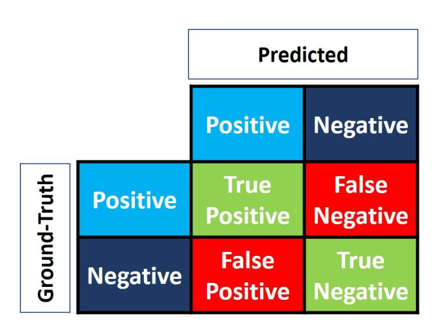
\includegraphics[width=0.8\linewidth]{pictures/Konfusionsmatrix_hs_analysis.png}
    \caption{Darstellung einer Konfusionsmatrix anhand von Annotationen (Ground-Truth) und Vorhersagen (Predicted) gemäß eines XNOR-Gatters}
    \label{fig:Konfusionsmatrix}
    \cite{noauthor_crc-modell_nodate}
\end{figure}


Precision 
\begin{equation}
    Precision = \frac{\mbox{\textit{correctly classified actual positives}}}{\mbox{\textit{everything classified as positive}}} = \frac{TP}{TP + FP}
\end{equation}

Die Präzision beträgt im Idealfall ebenfalls 1,0 und hängt von der Anzahl falsch positiver Ergebnisse ab. Je geringer diese ist, besto besser die Genauigkeit. Präzision und Recall stehen sich in der Form gegenüber, als dass sie ein umgekehrtes Verhältnis haben und in der Regel mit steigender Präzision der Recall abnimmt vice versa.


\begin{equation}
    Recall (\mbox{\textit{True Positive Rate, TPR}}) = \frac{\mbox{\textit{correctly classified actual positives}}}{\mbox{\textit{all actual positives}}} = \frac{TP}{TP + FN}
\end{equation}

Der Recall ist ein Indikator für die Erkennungswahrscheinlichkeit eines Modells, wobei ebenfalls ein Wert von 1,0 = 100\% angestrebt wird. Für die Anwendung an realen Datensätzen mit geringem Aufkommen positiver Ergebnisse bietet diese Berechnung mehr Aussagekraft als die Genauigkeit. Erfasst wird die Fähigkeit eines Modells zur richtigen Identifikation von positiven Instanzen.

\begin{equation}
    \mbox{\textit{FPR (False Positive Rate)}} = \frac{\mbox{\textit{incorrectly classified actual negatives}}}{\mbox{\textit{all actual negatives}}} = \frac{FP}{FP + TN}
\end{equation}

Die Wahrscheinlichkeit eines Fehlalarms, wie die Falsch-Positiv-Rate auch genannt wird, soll im Idealfall bei 0,0 und somit 0 \% liegen. Im Realfall ergibt sich die Aussagekraft aus der Anzahl von tatsächlichen Negativwerte und damit eine entsprechende Instabilität. 

F1-Score
\begin{equation}
    2 * \frac{Precision * Recall}{Precision + Recall}
\end{equation}

Der F1-Score liefert den harmonischen Mittelwert anstelle des arithmethischen aufgrund der stärkeren Gewichtung von großen Unterschieden. Mit niedriger Genauigkeit (Precision) oder Trefferquote (Recall) sinkt das Ergebnis selbst bei einem hohen Gegenwert.  

Im Wesentlichen werden also die Schwächen von Präzision und Recall miteinander verrechnet und darüber ausgewogen, was schwerer zu manipulierendes Resultat bedeutet. 

Accuracy 
\begin{equation}
    Accuracy = \frac{\mbox{\textit{correct classifications}}}{\mbox{\textit{total classifications}}} = \frac{TP + TN}{TP + TN + FP + FN}
\end{equation}

Die Genauigkeit beschreibt den Anteil aller korrekten Klassifizierungen unabhängig von wahr oder falsch. Dies kann bei einer ausgewogenen Verteilung von TP und TN als eine ungefähre Übersicht für die Modellqualität dienen. Im Idealfall würde ein perfektes Modell weder falsch positive noch falsch negative Ergebnisse produzieren, was einer hundertprozentigen Genauigkeit entsprechen würde.

Im Realfall liegen unausgewogene Datensätze vor, bei dem entweder FN oder FP als Fehler überwiegt und damit die Aussagekraft reduziert. Entsprechend würde bei einem seltenen Aufkommen einer Klasse von nur 1\% das Modell in 100\% der Fälle \say{negativ} Vorhersagen, was in 99\% korrekt und dennoch nutzlos wäre. 

Die Kürzel stehen für folgendes: TP = True Positive (wahre Positive), TN = True Negative (wahre Negative), FP = False Positive (falsche Positive) und FN = False Negative (falsche Negative).

Die Wahl fällt hier auf den harmonischen Mittelwert gegenüber des arithmethischen aufgrund der stärkeren Gewichtung von großen Unterschieden. Mit niedriger Genauigkeit (Precision) oder Trefferquote (Recall) wird sinkt das Ergebnis selbst bei einem hohen Gegenwert.  

Intersection over Union
\begin{equation}
    IoU = \frac{|A\cap B|}{|A\cup B|}
\end{equation}
Die Intersection over Union (zu Deutsch: Verhältnis der Schnittmenge zur Vereinigungsmenge, auch genannt Jaccard-Koeffizient) stellt ein Ähnlichkeitsmaß für Vektoren, Mengen und andere Objekte dar. Das dient der Beurteilung der Genauigkeit von Objekterkennungsmodellen und ihrer Optimierung. So definiert in \cite{goodfellow_2016}.

In der Form des Projekts stellt \textbf{IoU} die Schnittmenge der Ground Truth Pixelannotation und Vorhersage geteilt durch die Vereinigungsmenge derselben dar. Je ähnlicher Schnitt- und Vereinigungsmenge desto mehr nähert sich der Wert gleich eins. Während hierbei vollständige Übereinstimmung herrscht, ist diese bei null überhaupt nicht vorhanden. Es handelt sich also um eine prozentuale Gewichtung (?). Die \textbf{mIoU} -> \textbf{mean Intersection over Union} beschreibt den durchschnittlichen IoU über mehrere Objekterkennungen zur besseren Gesamtakkuranz eines Models. Da die Segmentierung pixelweise geschieht, ist der allgemeine Durchschnitt das beste Maß, solange das Objekt selbst keine Rolle spielt. 


\textbf{Quantisierung/Optimierung} für Edge-Geräte ergänzen (z.B. Post-Training Quantization, INT8/FP16, Latenz vs. Genauigkeit, Speicherbedarf; Bezug zu TensorFlow Lite).

Um den Anspruch an die Rechenressourcen zu reduzieren, wird \textbf{Post Training Quantization (PTQ)} eingesetzt. Damit hierbei keine Präzision verloren geht, wird die herkömmliche FP16 Aktivierungsausbreitung auf INT8 komprimiert. Das führt zu etwas g\cite{tensorflowPosttrainingQuantization}

\section{Theoretische Grundlagen}
\subsection{Neuronale Netze - Deep Learning}
Künstliche Intelligenz und Neuronale Netze stellen seit einigen Jahren den Status Quo dar, weswegen diese Technologie jedem ein Begriff sein sollte. Dennoch sei die grundlegende Funktionsweise hier erklärt, um das Basiswissen zu vereinheitlichen: 

Das sogennante \say{Deep-Learning} stellt, wie der Name es bereits andeutet, eine vertiefende Variante des machinellen Lernens dar. Während bei dieser veralteten Form noch Algorithmen definiert werden, die anhand mathematischer Logik Operationen explizit ausführen, werden bei der Tiefenlern-Methode. Mittels Verzerrungen und Gewichtungen des Modells kann das neuronale Netz auf der Basis von maschinellem Lernen optimiert werden, indem die Verknüpfung hinsichtlich ihrer Stärke angepasst werden. Während neuronale Netze und \say{Deep Learning} oft synonym verwendet werden, sind die Begriffe nicht ganz identisch. Per Definition liegt Deep Learning erst ab vier Schichten vor, obwohl moderne neuronale Netze diese Tiefe weit überschreiten.  \cite{goodfellow_2016} \\ \\

\begin{figure}
    \centering
    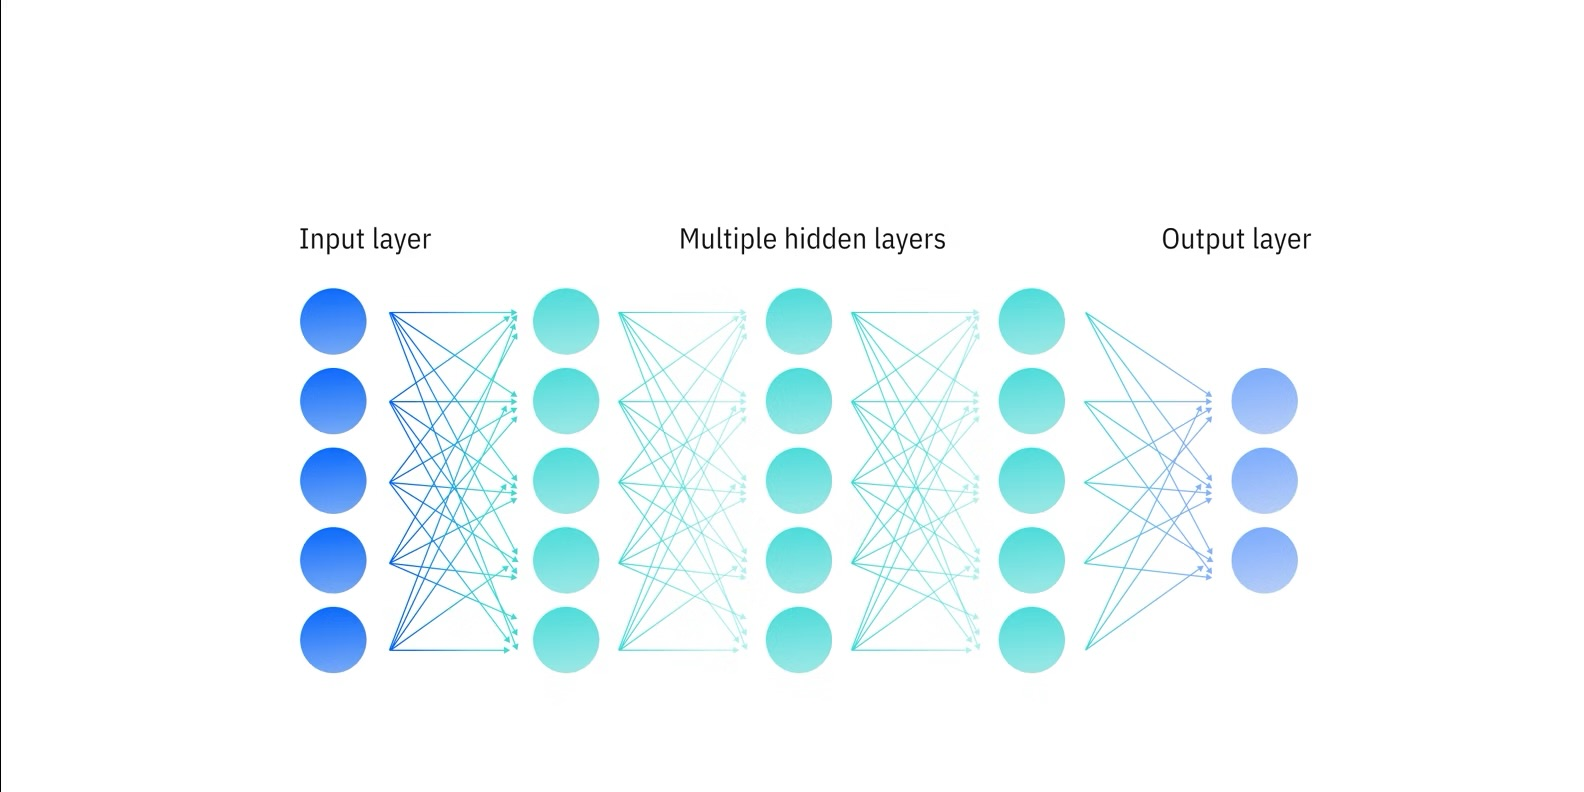
\includegraphics[width=0.5\linewidth]{pictures/deep-neural-network-diagram_2x1.png}
    \caption{}
    \label{fig:neural_network}
\end{figure}

Die unterschiedliche Funktionsweise von maschinellem Lernen und \say{Deep-Learning} lässt sich anhand dieses Gedankenexperiments darstellen: die Daten liegen als einzelne Punkte (x,y) in einem zweidimensionalen Koordinationsystem und sollen mittels Modelltrainings so verarbeitet werden, dass eine Linie diese erfasst. Während der klassische Lösungsansatz in der Definition einer Funktion liegt, die in Linien- oder Kurvenform dieses Ziel erreicht (machinelles Lernen), werden bei dem modernen Ansatz sämtliche Linien durch einzelne Punkte angepasst, rekombiniert und schließlich zu einer Form zusammengefügt. \cite{goodfellow_2016}

Aufgrund ihrer hohen Flexibilität werden neuronal Netze auch als ``universelle Approximatoren'' bezeichnet, da hypothetisch jede Funktion über eine neuronale Netzvereinbarung reproduziert werden kann.



\section{Convolutional Neural Network}

Ein Convolutional Neural Network (CNN oder ConvNet), zu deutsch ein faltbares neuronales Netzwerk, ist ein speziell für die Bild- und Videoverarbeitung ausgelegtes Konzept, was in seinen Grundstrukturen 1979 von Kunihiko Fukushima mit dem \say{Neocognitron} entwickelt und seitdem schrittweise verbessert wurde. 

Namensgebend sind die Convolutional Layer, die auf dem Prinzip der diskreten Faltung basieren. Hierfür wird mittels eines Filterkernels die Eingabe schrittweise verarbeitet und dieses innere Produkt wird an die Neuronen weitergeleitet. Aufgrund der Mehrfachverarbeitung von überlappenden Bereichen zeichnen sich Ähnlichkeiten bei benachbarten Neuronen ab. Das Training der jeweiligen Schicht an Neuronen ist hierbei auf den Inhalt der vorherigen Schicht beschränkt, was sich durch die Ursprünge aus den biologischen rezeptiven Feldern herleitet. Dabei werden im Wesentlichen Informationen aus einem Bereich an Sinnesrezeptoren über ein Neuron verarbeitet, was Vorteile in der biologischen Datenverarbeitung bietet. 
Ein weiterer relevanter Bestandteil sind die geteilten Gewichte sämtlicher Neuronen (shared weights), die eine Grundlage für die Erkennung von Kanten, Ecken und weiteren Basisformen bietet. Auch die jeweilige Intensität in der Detektion kann angepasst werden, was vor allem bei der Kantenerkennung als Grundlage in der Bilderkennung verwendet. 

\begin{figure}
    \centering
    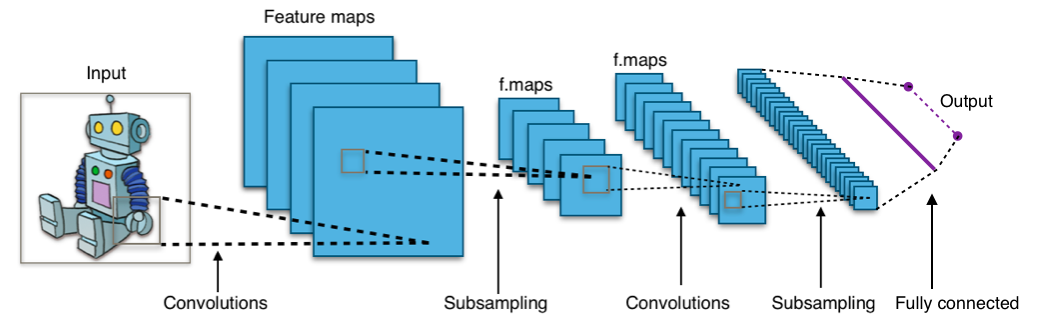
\includegraphics[width=1\linewidth]{pictures/Typical_cnn_wikimedia.png}
    \caption{Verarbeitung der Daten über mehrere Schichten des CNN}
    \label{fig:CNN_Layers}
\end{figure}

Weitergehend werden für gewöhnlich ReLUs und Backpropagation für die Konvertierung des Inputs zum Output verwendet. 
Mittels der Faltungsmatrix wird die regulär eine zwei- bis dreidimensionale Matrix als Input verarbeitet, was zu einer Aktivierung führt. Bei repetitiver Ausführung dieses Schritts zeichnet sich eine Feature Map als Karte dieser Aktivierungen ab. Mit Convolutional Layern werden mehrere dieser datensatzspezifischen Filter gleichzeitig erlernt und dadurch die Erkennung von typischen Merkmalen gestärkt.    

\section{MobileNetV3}

MobileNet ist ein leichtes Convolutional Neural Networks (CNN) von Howard et al das für den Einsatz auf mobilen Endgeräten entworfen wurde und entsprechend geringere Anforderungen im Vergleich zu ähnlichen Modellen aufweist. Ein Kernelement sind die depthwise separable convolutions. Diese ersetzen die konventionellen Convolutional Layer durch ein zweischichtiges System. Einerseits werden räumliche Tiefeninformationen grob und leichtgewichtig bearbeitet sowie zugleich konserviert, während im zweiten Layer eine aufwändigere punktweise 1x1 Faltung vorgenommen wird, die der Generierung von Eigenschaften gilt. Durch diese Trennung sinkt die Anzahl an Parameter und mathematische Operationen, während die Aussagekraft hoch bleibt. 

Verbessert wurde dieses Grundmodell mit Version 2 bei dem inverted residuals und linear bottlenecks eingeführt wurden. Bei invertierten Residuen handelt es sich um eine Möglichkeit des Netzwerks, Aktivierungen früher zu erreichen. Indem eine Verbindung zwischen Anfang und Ende eines Convolutional Blockes geschaffen wird, können Hochskalierungen übersprungen und damit Parameter eingespart werden, was sich für das Training von tiefen Netzen als äußerst effizient herausgestellt hat.   
Andererseits werden hierdurch Leistungseinbußen verursacht, die an anderer Stelle korrigiert werden mit linearen Flaschenhälsen. Dafür werden 1x1 Layer zwischen den restlichen Schichten in die building blocks für In- und Output eingebaut, die die Eingabe auf das Format reduzieren und somit harmonisieren. Die Blöcke der layer transformation bestehen weiterhin aus einer nicht linearen Funktion, was die Vorteile beider Varianten bedeutet.
\cite{}

\begin{figure}[h]
    \centering
    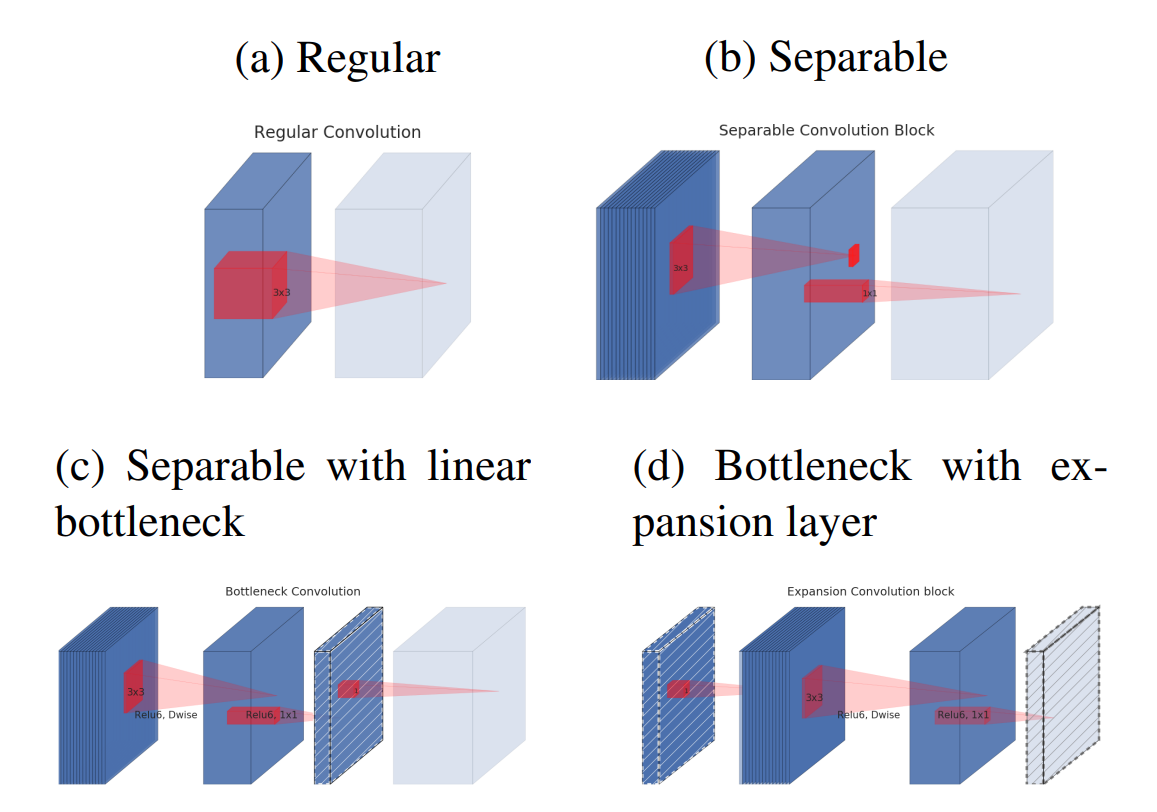
\includegraphics[width=0.6\linewidth]{pictures/MobileNetV2_Convolutions_og_paper.png}
    \caption{Darstellung der unterschiedlichen Varianten von Convolutions mit den Merkmalen von MobileNet}
    \label{fig:convolutions}
\end{figure}

\begin{figure}[]
    \centering
    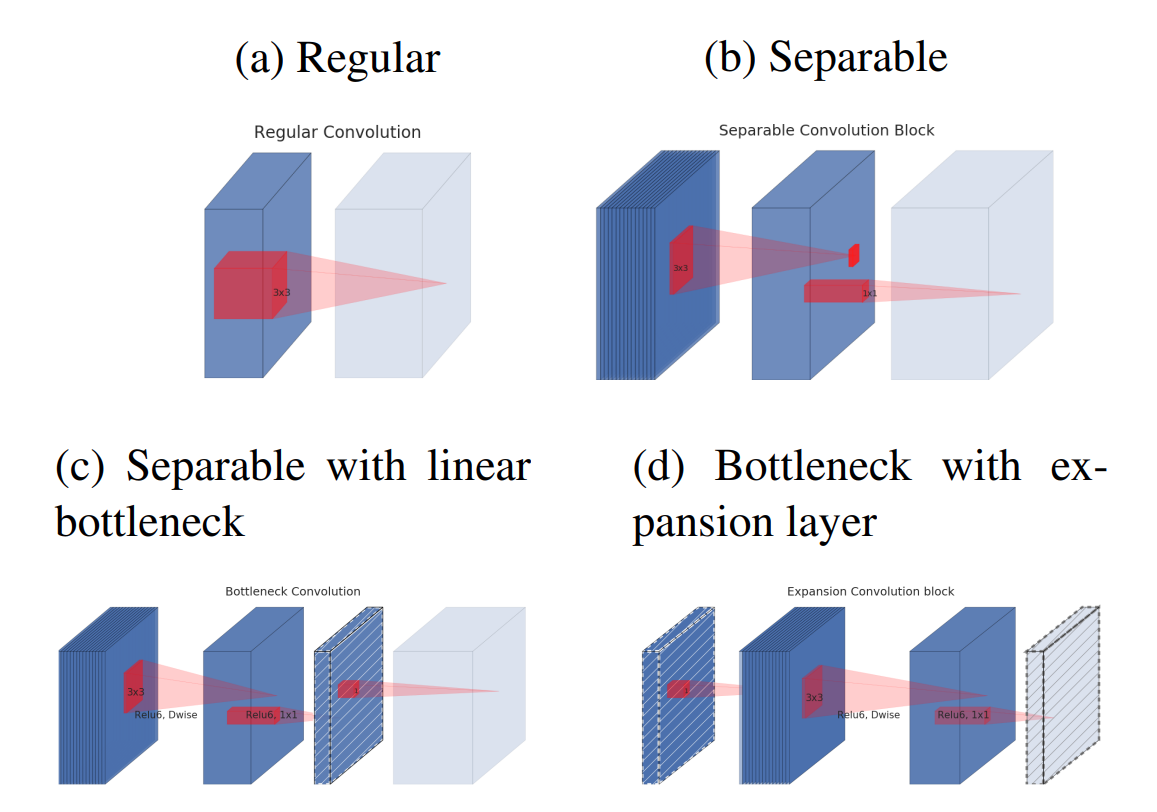
\includegraphics[width=0.8\linewidth]{pictures/MobileNetV2_Convolutions_og_paper.png}
    \caption{Darstellung der unterschiedlichen Varianten von Convolutions mit den Merkmalen von MobileNet}
    \label{fig:convolutions}
\end{figure}

\textbf{Quelle zur Abbildung ergänzen} und korrekt zitieren (\texttt{\textbackslash cite\{...\}}); leere Zitation entfernen, sonst Bibliographiefehler.

Im Rahmen der MobileNet Version V3 wurden die bestehenden ReLUs durch swish nonlinearity Funktionen ersetzt, die eine Kombination aus einfacher und harter Sigmoid-Funktion darstellt. 
Darüber hinaus wurde die Plattformerkennung mittels NAS optimiert, ein Netzwerk-Feintuning durch NetAdapt und Squeeze-and-Excite (SE) Module hinzugefügt.



\section{Zusammenfassung/Bewertung}
Aufgrund der vielseitigen Anforderungen an das Projekt hinsichtlich der Umgebung, Sicherheitsanforderungen und Zeitrahmens stellt ein auf Raspberry Pi 5 basierendes System mit MobileNetV3 unter TF-Lite Runtime die beste Alternative dar. Hiermit gestaltet sich der hochwertigste Trade-Off zwischen Perfomanz, Simplizität und Kosten. Das zugrunde liegende CNN in Kombination mit Semantischer Segmentierung ist zwar eine aufwändigere Form durch die notwendige Pixelannotation, bietet aber Vorteile durch simple Grenzwertbestimmung, die für das Schaltverhalten der Peripherie sinnvoll ist. Der Raspberry stellt durch die Vielfalt an Online-Anleitungen und direkte physische Anbindung per GPIO-Pins den optimalen Kompromiss aus DIY- und Industrielösung dar, ohne einen Mikrocontroller zu benötigen. 


\ldots